\documentclass[border=10pt]{standalone}
\usepackage{tikz}
\usepackage{xcolor}
\usetikzlibrary{shapes,arrows.meta,positioning,calc,shadows,backgrounds,fit}

% Colors
\definecolor{psychpurple}{RGB}{155,89,182}
\definecolor{behaviorblue}{RGB}{52,152,219}
\definecolor{socialgreen}{RGB}{46,204,113}
\definecolor{cognitiveorange}{RGB}{230,126,34}
\definecolor{consumerred}{RGB}{231,76,60}
\definecolor{lightgray}{RGB}{245,245,245}
\definecolor{darktext}{RGB}{50,50,50}

\begin{document}
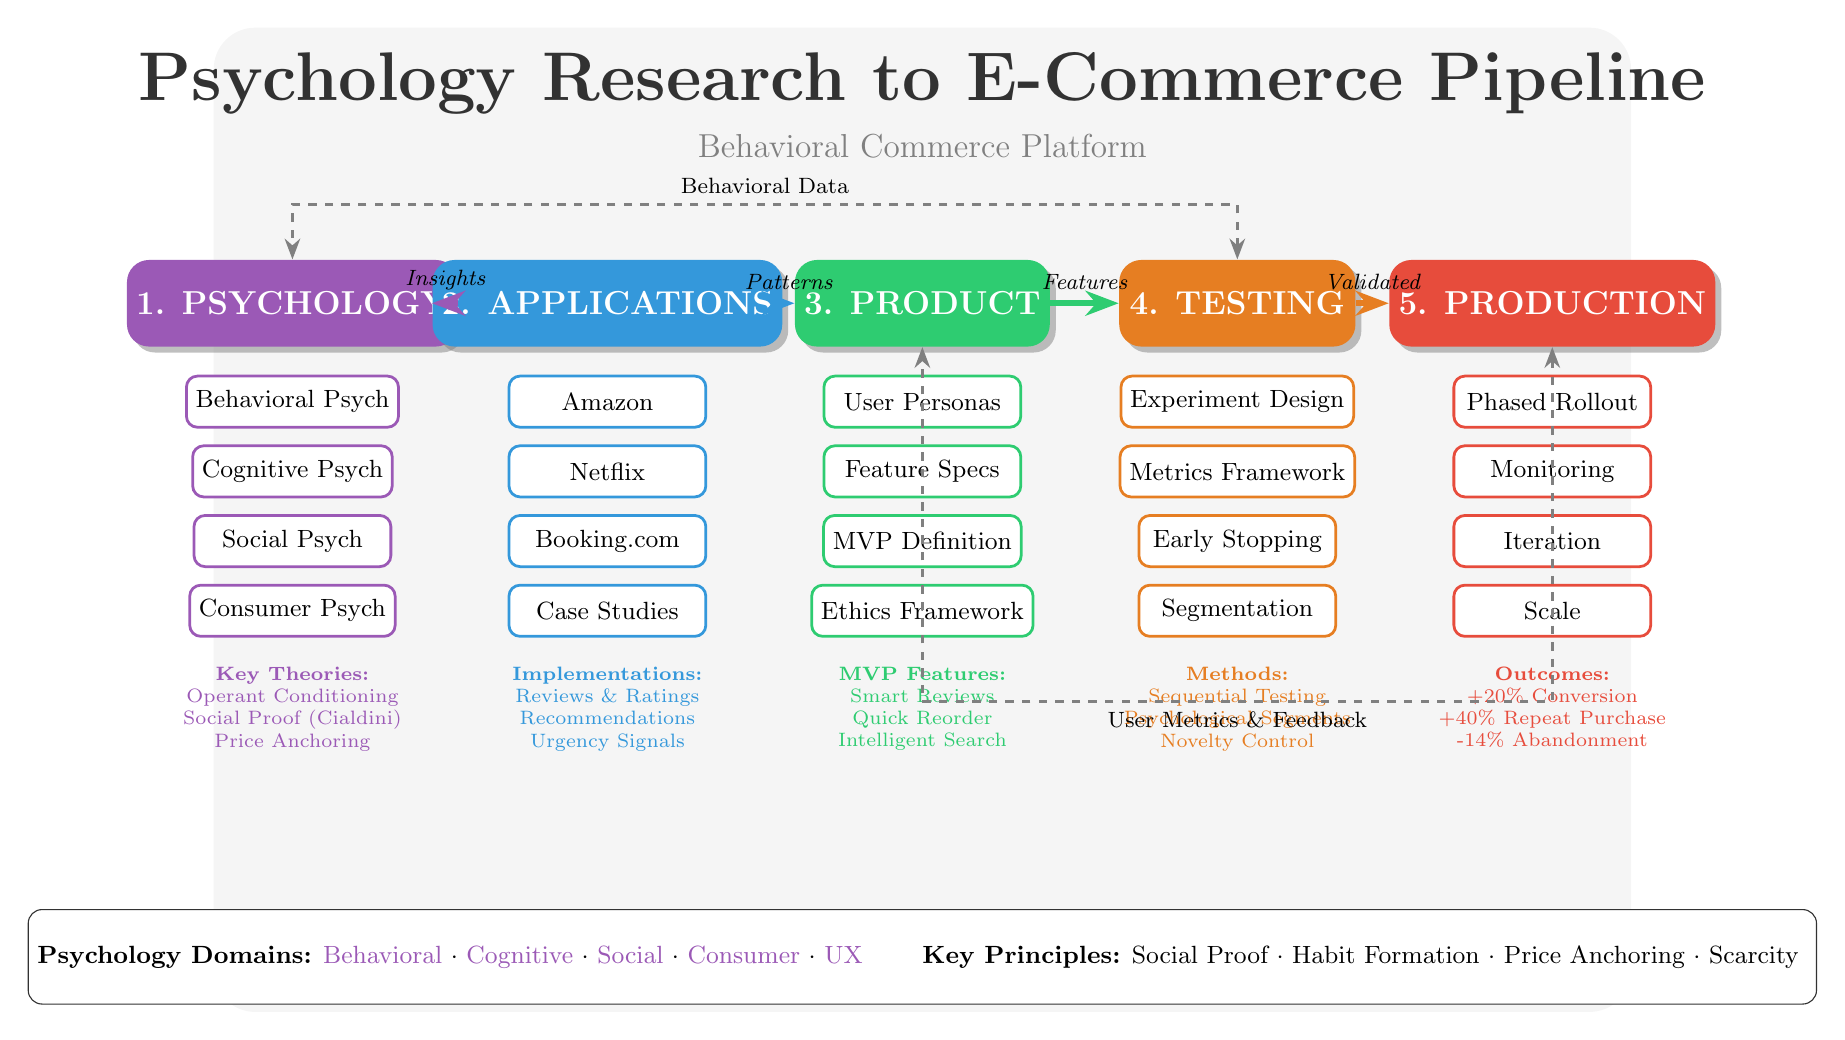
\begin{tikzpicture}[
    phase/.style={
        rectangle,
        rounded corners=8pt,
        minimum width=3cm,
        minimum height=1.1cm,
        text centered,
        font=\bfseries\large,
        text=white,
        drop shadow
    },
    subnode/.style={
        rectangle,
        rounded corners=4pt,
        minimum width=2.5cm,
        minimum height=0.65cm,
        text centered,
        font=\small,
        fill=white,
        draw=#1,
        line width=1pt
    },
    arrow/.style={
        ->,
        >=Stealth,
        line width=2pt,
        draw=darktext
    },
    feedback/.style={
        <->,
        >=Stealth,
        line width=1pt,
        draw=gray,
        dashed
    }
]

% Background
\begin{scope}[on background layer]
    \fill[lightgray, rounded corners=15pt] (-1,-8) rectangle (17,4.5);
\end{scope}

% Title
\node[font=\Huge\bfseries, text=darktext] at (8,3.8) {Psychology Research to E-Commerce Pipeline};
\node[font=\large, text=gray] at (8,3) {Behavioral Commerce Platform};

%==============================================================================
% PHASE 1: PSYCHOLOGY RESEARCH
%==============================================================================
\node[phase, fill=psychpurple] (research) at (0,1) {1. PSYCHOLOGY};

\node[subnode=psychpurple, below=0.35cm of research] (behav) {Behavioral Psych};
\node[subnode=psychpurple, below=0.2cm of behav] (cog) {Cognitive Psych};
\node[subnode=psychpurple, below=0.2cm of cog] (social) {Social Psych};
\node[subnode=psychpurple, below=0.2cm of social] (consumer) {Consumer Psych};

\node[font=\scriptsize, text=psychpurple, below=0.25cm of consumer, align=center] {
    \textbf{Key Theories:}\\
    Operant Conditioning\\
    Social Proof (Cialdini)\\
    Price Anchoring
};

%==============================================================================
% PHASE 2: INDUSTRY APPLICATIONS
%==============================================================================
\node[phase, fill=behaviorblue] (apps) at (4,1) {2. APPLICATIONS};

\node[subnode=behaviorblue, below=0.35cm of apps] (amazon) {Amazon};
\node[subnode=behaviorblue, below=0.2cm of amazon] (netflix) {Netflix};
\node[subnode=behaviorblue, below=0.2cm of netflix] (booking) {Booking.com};
\node[subnode=behaviorblue, below=0.2cm of booking] (cases) {Case Studies};

\node[font=\scriptsize, text=behaviorblue, below=0.25cm of cases, align=center] {
    \textbf{Implementations:}\\
    Reviews \& Ratings\\
    Recommendations\\
    Urgency Signals
};

%==============================================================================
% PHASE 3: PRODUCT STRATEGY
%==============================================================================
\node[phase, fill=socialgreen] (product) at (8,1) {3. PRODUCT};

\node[subnode=socialgreen, below=0.35cm of product] (personas) {User Personas};
\node[subnode=socialgreen, below=0.2cm of personas] (features) {Feature Specs};
\node[subnode=socialgreen, below=0.2cm of features] (mvp) {MVP Definition};
\node[subnode=socialgreen, below=0.2cm of mvp] (ethics) {Ethics Framework};

\node[font=\scriptsize, text=socialgreen, below=0.25cm of ethics, align=center] {
    \textbf{MVP Features:}\\
    Smart Reviews\\
    Quick Reorder\\
    Intelligent Search
};

%==============================================================================
% PHASE 4: A/B TESTING
%==============================================================================
\node[phase, fill=cognitiveorange] (testing) at (12,1) {4. TESTING};

\node[subnode=cognitiveorange, below=0.35cm of testing] (design) {Experiment Design};
\node[subnode=cognitiveorange, below=0.2cm of design] (metrics) {Metrics Framework};
\node[subnode=cognitiveorange, below=0.2cm of metrics] (stopping) {Early Stopping};
\node[subnode=cognitiveorange, below=0.2cm of stopping] (segment) {Segmentation};

\node[font=\scriptsize, text=cognitiveorange, below=0.25cm of segment, align=center] {
    \textbf{Methods:}\\
    Sequential Testing\\
    Psychological Segments\\
    Novelty Control
};

%==============================================================================
% PHASE 5: PRODUCTION
%==============================================================================
\node[phase, fill=consumerred] (prod) at (16,1) {5. PRODUCTION};

\node[subnode=consumerred, below=0.35cm of prod] (rollout) {Phased Rollout};
\node[subnode=consumerred, below=0.2cm of rollout] (monitor) {Monitoring};
\node[subnode=consumerred, below=0.2cm of monitor] (iterate) {Iteration};
\node[subnode=consumerred, below=0.2cm of iterate] (scale) {Scale};

\node[font=\scriptsize, text=consumerred, below=0.25cm of scale, align=center] {
    \textbf{Outcomes:}\\
    +20\% Conversion\\
    +40\% Repeat Purchase\\
    -14\% Abandonment
};

%==============================================================================
% MAIN FLOW ARROWS
%==============================================================================
\draw[arrow, draw=psychpurple] (research.east) -- (apps.west);
\draw[arrow, draw=behaviorblue] (apps.east) -- (product.west);
\draw[arrow, draw=socialgreen] (product.east) -- (testing.west);
\draw[arrow, draw=cognitiveorange] (testing.east) -- (prod.west);

% Labels
\node[font=\footnotesize\itshape, above=0.05cm] at ($(research.east)!0.5!(apps.west)$) {Insights};
\node[font=\footnotesize\itshape, above=0.05cm] at ($(apps.east)!0.5!(product.west)$) {Patterns};
\node[font=\footnotesize\itshape, above=0.05cm] at ($(product.east)!0.5!(testing.west)$) {Features};
\node[font=\footnotesize\itshape, above=0.05cm] at ($(testing.east)!0.5!(prod.west)$) {Validated};

%==============================================================================
% FEEDBACK LOOPS
%==============================================================================
\draw[feedback]
    (testing.north) -- ++(0,0.7) -|
    node[pos=0.25, above, font=\footnotesize] {Behavioral Data}
    (research.north);

\draw[feedback]
    (prod.south) -- ++(0,-4.5) -|
    node[pos=0.25, below, font=\footnotesize] {User Metrics \& Feedback}
    (product.south);

%==============================================================================
% KEY BOX
%==============================================================================
\node[draw=darktext, rounded corners=5pt, fill=white,
      minimum width=15cm, minimum height=1.2cm,
      font=\small, align=center] at (8,-7.3) {
    \textbf{Psychology Domains:}
    \textcolor{psychpurple}{Behavioral} $\cdot$
    \textcolor{psychpurple}{Cognitive} $\cdot$
    \textcolor{psychpurple}{Social} $\cdot$
    \textcolor{psychpurple}{Consumer} $\cdot$
    \textcolor{psychpurple}{UX}
    \quad\quad
    \textbf{Key Principles:}
    Social Proof $\cdot$ Habit Formation $\cdot$ Price Anchoring $\cdot$ Scarcity
};

\end{tikzpicture}
\end{document}
